L'organisation de données non structurées comme du texte présente des défis importants.
Les bases de données sont des structures complexes dont l'apparence peut différer considérablement.
Cependant, on retrouve toujours une structure intrinsèque composée des données nommées (ou attributs) organisé en groupe (tuples ou nœuds) eux même regrouper par type (table ou label).
On identifie aussi certains groupes spéciaux qui connecte des groupes entre eux et qu'on appelle relations.
C'est le fondement du \gls{mea} \cite{chenEntityrelationshipModelUnified1976}.
Il en va de même pour les textes qui possèdent plusieurs structures.
La grammaire du français ou de l'anglais définit comment les phrases doivent être construites.
L'idée est de pouvoir permettre la transformation de la grammaire du texte vers une autre (celle du \gls{mea}).

\cite{barretGenericAbstractionsData2021} se base sur le \gls{mea} pour identifier des connexions entre des jeux de données hétérogènes.
Les auteurs introduisent la notion de \emph{sub-record} pour une donnée, de \emph{record} pour les groupements de données et de collections, reliés entre eux sous forme d'arborescence.
Dans ce modèle, un jeu de données forme donc un arbre.
Chaque type de nœud est associé à une sémantique : un \emph{record} ne peux avoir que des \emph{sub-record} comme enfants, une collection est hétérogène et ne peux donc pas contenir différents \emph{records}.

\begin{definition}[Structure de donnée universelle]
    Si une instance $I$ est un arbre, ce dernier est reconnu par une grammaire $G_S$ qui est le schéma de l'instance.
    Ici, on traitera $I$ comme un arbre de dérivation de $G_S$, la grammaire est donc une \gls{cfg} et non une grammaire d'arbre.
    Cependant, un schéma n'est valide que s'il est de la forme \gls{mea} et qu'il respecte les règles sémantiques décrites dans \cite{barretGenericAbstractionsData2021}.
    C'est-à-dire que l'on peut définir une méta-grammaire $G$ qui reconnait l'ensemble des grammaires de schéma valides.
    $G$ est défini comme une méta-grammaire S-attribuée et est donnée figure~\ref{table:struct:meta} en utilisant la \gls{bnf}.
    $\langle X_A \rangle$ est un méta-non-terminaux avec pour attributs l'ensemble $A$, $\textsc{eol}$ est le séparateur entre les règles de la grammaire de destination et on retrouve à droite de chaque règle de production l'ensemble de formule sémantique $\Phi$.
    Les attributs sont définis comme suit :
    \begin{itemize}
        \item $name$, $grpName$, $relName$ sont des attributs qui prennent le nom d'une instance d'un non-terminal. Par exemple, pour le non-terminal $ENT$ on peut obtenir dans la grammaire de destination les instances $ENT_{person}$ et $ENT_{exam}$
        \item $eL$ est un ensemble de nom d'entités
        \item $gL$ est un ensemble de nom de groupes
        \item $cgL$ est un ensemble de nom de collection de groupes
        \item $rL$ est un ensemble de nom de relations
        \item $crL$ est un ensemble de nom de collection de relations
    \end{itemize}
    Dans la méta-grammaires ces attributs servent (en plus de la validation des formules sémantiques) à garder une trace des règles de production qui ont été construite afin de vérifier que les grammaires produites sont valides, c.-à-d. que tout non-terminal qui apparait dans une règle de production est bien défini dans une autre règle.
\end{definition}

\begin{example}
    Étant donné un schéma définit par la grammaire $G_S$ suivante :
    \begin{align*}
        ROOT    & \to GROUP_A ~ COLL_1     \\
        COLL_1  & \to REL_X^+              \\
        REL_X   & \to GROUP_A ~ GROUP_B    \\
        GROUP_A & \to ENT_1                \\
        GROUP_B & \to ENT_1 ~ ENT_2        \\
        ENT_1   & \to \langle data \rangle \\
        ENT_2   & \to \langle data \rangle
    \end{align*}

    L'arbre de dérivation de $G$ donnant $G_S$ est donné figure~\ref{table:struct:meta:ex}.
    En bleu on note, pour chaque nœud, la valeur de chaque attribut en omettant, pour des raisons de visibilité, les attributs ayant pour valeur un ensemble vide.
\end{example}

\begin{landscape}
    \centering
    \begin{adjustbox}{max width=\linewidth,max height=.95\textheight,valign=c}
        \parbox{\linewidth}{\begin{align}
                \epsilon                                     & ::= \langle root_{eL',gL',cgL',rL',crL'} \rangle ~\textsc{eol}~ \langle ruleList_{eL,gL,cgL,rL,crL} \rangle  & [eL' \subseteq eL; gL' \subseteq gL; cgL' \subseteq cgL; rL' \subseteq rL; crL' \subseteq crL]         \\
                \langle root_{eL,gL,cgL,rL,crL} \rangle      & ::= ROOT \to \langle rootList_{eL,gL,cgL,rL,crL} \rangle                                                                                                                                                              \\[1em]
                % Root list
                \langle rootList_{eL,gL,cgL,rL,crL}  \rangle & ::= \epsilon                                                                                                 & [eL \gets \emptyset; gL \gets \emptyset; cgL \gets \emptyset; rL \gets \emptyset; crL \gets \emptyset] \\
                                                             & ~~ \mid ~  ENT_{name}   ~ \langle rootList_{eL',gL,cgL,rL,crL} \rangle                                       & [name \notin eL'; eL \gets \{name\} \cup eL']                                                          \\
                                                             & ~~ \mid ~  GROUP_{name} ~ \langle rootList_{eL,gL',cgL,rL,crL} \rangle                                       & [name \notin gL'; gL \gets \{name\} \cup gL']                                                          \\
                                                             & ~~ \mid ~  REL_{name}   ~ \langle rootList_{eL,gL,cgL,rL',crL} \rangle                                       & [name \notin rL'; rL \gets \{name\} \cup rL']                                                          \\
                                                             & ~~ \mid ~  COLL_{name}  ~ \langle rootList_{eL,gL,cgL',rL,crL} \rangle                                       & [name \notin cgL'; cgL \gets \{name\} \cup cgL']                                                       \\
                                                             & ~~ \mid ~  COLL_{name}  ~ \langle rootList_{eL,gL,cgL,rL,crL'} \rangle                                       & [name \notin crL'; crL \gets \{name\} \cup crL']                                                       \\[1em]
                % Rules list
                \langle ruleList_{eL,gL,cgL,rL,crL}  \rangle & ::= \epsilon                                                                                                 & [eL \gets \emptyset; gL \gets \emptyset; cgL \gets \emptyset; rL \gets \emptyset; crL \gets \emptyset] \\
                                                             & ~~ \mid ~ \langle entity_{name}          \rangle ~\textsc{eol}~ \langle ruleList_{eL',gL,cgL,rL,crL} \rangle & [name \notin eL'; eL \gets \{name\} \cup eL']                                                          \\
                                                             & ~~ \mid ~ \langle group_{name, eL'}      \rangle ~\textsc{eol}~ \langle ruleList_{eL,gL',cgL,rL,crL} \rangle & [name \notin gL'; eL' \subseteq eL; gL \gets \{name\} \cup gL']                                        \\
                                                             & ~~ \mid ~ \langle relation_{name, gL'}   \rangle ~\textsc{eol}~ \langle ruleList_{eL,gL,cgL,rL',crL} \rangle & [name \notin rL'; gL' \subseteq gL; rL \gets \{name\} \cup rL']                                        \\
                                                             & ~~ \mid ~ \langle collGrp_{name,grpName} \rangle ~\textsc{eol}~ \langle ruleList_{eL,gL,cgL',rL,crL} \rangle & [name \notin cgL'; grpName \in gL; cgL \gets \{name\} \cup cgL']                                       \\
                                                             & ~~ \mid ~ \langle collRel_{name,relName} \rangle ~\textsc{eol}~ \langle ruleList_{eL,gL,cgL,rL,crL'} \rangle & [name \notin crL'; relName \in rL; crL \gets \{name\} \cup crL']                                       \\[1em]
                % Groups
                \langle group_{name, eL} \rangle             & ::= GROUP_{name} \to \langle entList_{eL} \rangle                                                                                                                                                                     \\
                \langle collGrp_{name,grpName} \rangle       & ::= COLL_{name} \to GROUP_{grpName}^+                                                                                                                                                                                 \\[1em]
                % Relations
                \langle relation_{name, gL} \rangle          & ::= REL_{name} \to GROUP_{name1} ~ GROUP_{name2}                                                             & [gL \gets \{name1, name2\}; name1 \neq name2]                                                          \\
                \langle collRel_{name,relName} \rangle       & ::= COLL_{name} \to REL_{relName}^+                                                                                                                                                                                   \\[1em]
                % Entities
                \langle entList_{eL} \rangle                 & ::= ENT_{name}                                                                                               & [eL \gets \{name\}]                                                                                    \\
                                                             & ~~ \mid ~ ENT_{name} ~ \langle entList_{eL'} \rangle                                                         & [eL \gets \{name\} \cup eL'; name \notin eL']                                                          \\
                \langle entity_{name} \rangle                & ::= ENT_{name} \to \langle data \rangle
            \end{align}}
    \end{adjustbox}
    \captionof{table}{Méta-grammaire S-attribuée $G$ des schémas de base de donnée au format \glsname*{bnf} \label{table:struct:meta}}
\end{landscape}

\begin{landscape}
    \centering
    \vspace*{\fill}
    \begin{adjustbox}{max width=\linewidth,max height=.95\textheight,valign=c}
        \begin{forest}
            for tree={align=center}
            [\huge{$\epsilon$}
                [{\large{$\langle root \rangle$}\\$\color{blue}crL=\{1\}$\\$\color{blue}gL=\{A\}$}
                    [$ROOT$]
                    [$\to$,before computing xy={s/.average={s}{siblings}}]
                    [{\large{$\langle rootList \rangle$}\\$\color{blue}crL=\{1\}$\\$\color{blue}gL=\{A\}$}
                        [$GROUP_A$]
                        [{\large{$\langle rootList \rangle$}\\$\color{blue}crL=\{1\}$}
                            [$COLL_1$]
                            [\large{$\langle rootList \rangle$}
                                [$\epsilon$]
                            ]
                        ]
                    ]
                ]
                [\textsc{eol},before computing xy={s/.average={s}{siblings}}]
                [{\large{$\langle ruleList \rangle$}\\$\color{blue}crL=\{1\}$\\$\color{blue}rL=\{X\}$\\$\color{blue}gL=\{A, B\}$\\$\color{blue}eL=\{1, 2\}$}
                    [{\large{$\langle collRel \rangle$}\\$\color{blue}name=1$\\$\color{blue}relName=X$}
                        [$COLL_1$]
                        [$\to$,before computing xy={s/.average={s}{siblings}}]
                        [$REL_X^+$]
                    ]
                    [\textsc{eol},before computing xy={s/.average={s}{siblings}}]
                    [{\large{$\langle ruleList \rangle$}\\$\color{blue}rL=\{X\}$\\$\color{blue}gL=\{A, B\}$\\$\color{blue}eL=\{1, 2\}$}
                        [{\large{$\langle relation \rangle$}\\$\color{blue}name=X$\\$\color{blue}gL=\{A, B\}$}
                            [$REL_X$]
                            [$\to$]
                            [$GROUP_A$]
                            [$GROUP_B$]
                        ]
                        [\textsc{eol},before computing xy={s/.average={s}{siblings}}]
                        [{\large{$\langle ruleList \rangle$}\\$\color{blue}gL=\{A, B\}$\\$\color{blue}eL=\{1, 2\}$}
                            [{\large{$\langle group \rangle$}\\$\color{blue}name=A$\\$\color{blue}eL=\{1\}$}
                                [$GROUP_A$]
                                [$\to$,before computing xy={s/.average={s}{siblings}}]
                                [{\large{$\langle entList \rangle$}\\$\color{blue}eL=\{1\}$}
                                    [$ENT_1$]
                                ]
                            ]
                            [\textsc{eol},before computing xy={s/.average={s}{siblings}}]
                            [{\large{$\langle ruleList \rangle$}\\$\color{blue}gL=\{B\}$\\$\color{blue}eL=\{1, 2\}$}
                                [{\large{$\langle group \rangle$}\\$\color{blue}name=B$\\$\color{blue}eL=\{1, 2\}$}
                                    [$GROUP_B$]
                                    [$\to$,before computing xy={s/.average={s}{siblings}}]
                                    [{\large{$\langle entList \rangle$}\\$\color{blue}eL=\{1, 2\}$}
                                        [$ENT_1$]
                                        [{\large{$\langle entList \rangle$}\\$\color{blue}eL=\{2\}$}
                                            [$ENT_2$]
                                        ]
                                    ]
                                ]
                                [\textsc{eol},before computing xy={s/.average={s}{siblings}}]
                                [{\large{$\langle ruleList \rangle$}\\$\color{blue}eL=\{1, 2\}$}
                                    [{\large{$\langle ent \rangle$}\\$\color{blue}name=1$}
                                        [$ENT_1$]
                                        [$\to$]
                                        [$\langle data \rangle$]
                                    ]
                                    [\textsc{eol},before computing xy={s/.average={s}{siblings}}]
                                    [{\large{$\langle ruleList \rangle$}\\$\color{blue}eL=\{2\}$}
                                        [{\large{$\langle ent \rangle$}\\$\color{blue}name=2$}
                                            [$ENT_2$]
                                            [$\to$]
                                            [$\langle data \rangle$]
                                        ]
                                        [\textsc{eol},before computing xy={s/.average={s}{siblings}}]
                                        [\large{$\langle ruleList \rangle$}
                                            [$\epsilon$]
                                        ]
                                    ]
                                ]
                            ]
                        ]
                    ]
                ]
            ]
        \end{forest}
    \end{adjustbox}
    \captionof{figure}{Exemple de dérivation de la méta-grammaire \label{table:struct:meta:ex}}
    \vspace*{\fill}
\end{landscape}

\subsection{Textes et arbres}

Les textes possèdent une structure complexe, cependant il est possible de représenter un texte comme un arbre en utilisant une analyse syntaxique.
Ils existent deux structures très utilisées dans la littérature :

\begin{description}
    \item[Arbre syntaxique]
          (Figure~\ref{fig:struct:ex-tree:syx})
          C'est l'arbre de dérivation de la grammaire du texte.
          Il représente les relations syntaxiques (de proche en proche) entre les mots et les clauses et met en évidence la composition d'une phrase en sous partie.
          Les feuilles de l'arbre sont les unités lexicales (les mots) et les nœuds intermédiaires représente les structures abstraites comme une phrase verbales ou un groupe nominal.
          Chaque mot a pour parent un nœud représentant sa nature où \gls{pos} en anglais (nom, verbe, adjectif, etc).

    \item[Arbre de dépendance]
          (Figure~\ref{fig:struct:ex-tree:dep})
          Cette représentation met en évidence des liens syntaxique direct entre les unités lexicales représentant une forme de sémantique.
          Dans l'arbre de dépendance, chaque unité lexicale est un nœud de l'arbre et les arêtes sont labellisés par des relations syntaxiques comme sujet ou objet (entre un nom et un verbe), ou encore modifier entre un adjectif et un nom.
          Cet arbre est souvent utilisé dans les taches d'extraction d'information pour récupérer une sémantique entre les mots notamment, car des liens peuvent exister entre des mots très éloignés ce qui est moins évidents dans un arbre syntaxique.
\end{description}

\begin{figure}[ht]
    \centering
    \begin{subfigure}{\textwidth}
        \centering
        \begin{adjustbox}{max width=\linewidth}
            \begin{forest}
                where n children=0{tier=word}{}
                [S
                    [NP
                            [DT [la]]
                            [NP,before computing xy={s/.average={s}{siblings}} [fréquence]]
                            [NP [cardiaque]]
                    ]
                    [VP
                            [VBD [était]]
                            [PP
                                    [IN [à]]
                                    [NP
                                            [CD [100]]
                                            [NN [bpm]]
                                    ]
                            ]
                    ]
                ]
            \end{forest}
        \end{adjustbox}
        \caption{Arbre syntaxique}
        \label{fig:struct:ex-tree:syx}
    \end{subfigure}
    \begin{subfigure}{\textwidth}
        \centering
        \begin{adjustbox}{max width=\linewidth}
            \begin{dependency}
                \begin{deptext}[column sep=2em]
                    la \& fréquence \& cardiaque \& était \& à \& 100 \& b/min \\
                \end{deptext}
                \deproot{7}{root}
                \depedge{2}{1}{det}
                \depedge{2}{3}{amd}
                \depedge{7}{4}{cop}
                \depedge{7}{6}{nummod}
                \depedge{6}{5}{case}
                \depedge{7}{2}{nsubj}
            \end{dependency}
        \end{adjustbox}
        \caption{Arbre de dépendance}
        \label{fig:struct:ex-tree:dep}
    \end{subfigure}
    \caption[Comparaison entre l'arbre syntaxique et l'arbre de dépendance]{Comparaison entre l'arbre syntaxique (obtenu avec \gls{corenlp}) et l'arbre de dépendance (obtenu avec \gls{spacy}) pour la phrase \enquote{\textelp{} la fréquence cardiaque était à 100 b/min} issue du corpus CAS \cite{grabarCASFrenchCorpus2018}}
    \label{fig:struct:ex-tree}
\end{figure}

Pour la structuration automatique du texte, l'arbre de syntaxe est plus adapté, car sa structure est plus proche de la grammaire de destination même si l'on perd une partie de la sémantique exprimée par l'arbre de dépendance.
Les textes médicaux possèdent des phrases courtes et factuelles : les observations montrent que les éléments liés sémantiquement sont proches dans le texte \cite{savaryRelationExtractionClinical2022} ce qui mitige le manque de sémantique exprimé par l'arbre syntaxique.

\subsubsection{Conjonctions de coordinations}

\begin{figure}[ht]
    \centering
    \begin{subfigure}{.45\textwidth}
        \centering
        \begin{adjustbox}{max width=\linewidth}
            \begin{forest}
                where n children=0{tier=word}{}
                [NP
                    [DT [une]]
                    [NN [echographie]]
                    [ADJ [renale]]
                    [COORD
                            [CCONJ [et]]
                            [NP
                                    [DT [une]]
                                    [NN,before computing xy={s/.average={s}{siblings}} [cystographie]]
                                    [ADJ [retrograde]]
                            ]
                    ]
                ]
            \end{forest}
        \end{adjustbox}
        \caption{Conjonction en français}
        \label{fig:struct:conj:fr}
    \end{subfigure}
    \hfill
    \begin{subfigure}{.45\textwidth}
        \centering
        \begin{adjustbox}{max width=\linewidth}
            \begin{forest}
                where n children=0{tier=word}{}
                [COORD
                    [NP
                            [DT [a]]
                            [ADJ,before computing xy={s/.average={s}{siblings}} [renal]]
                            [NN [ultrasound]]
                    ]
                    [CCONJ,before computing xy={s/.average={s}{siblings}} [and]]
                    [NP
                            [DT [a]]
                            [ADJ,before computing xy={s/.average={s}{siblings}} [retrograde]]
                            [NN [cystography]]
                    ]
                ]
            \end{forest}
        \end{adjustbox}
        \caption{Conjonction en anglais}
        \label{fig:struct:conj:en}
    \end{subfigure}
    \caption{Comparaison entre les conjonctions en français et en anglais}
    \label{fig:struct:conj}
\end{figure}

\subsubsection{Enrichissement des arbres}

\subsubsection{Simplifications}

\subsection{Récupération du schéma d'une instance}

Pour réaliser la migration de l'instance d'une grammaire vers une autre il est indispensable de pouvoir récupérer la grammaire à partir de l'instance afin de pouvoir la vérifier à l'aide de la méta-grammaire $G$.
Étant donné une instance $I$ reconnu par une grammaire $G_S$, il est possible de récupérer l'arbre de dérivation $S$ de la grammaire $G$ en calculant le quotient de $I$. \todo{$S$ n'est pas la dérivation de $G$}

\begin{definition}[Quotient d'un graphe]
    Étant donné un graphe $G = (V, E)$ où $V$ est l'ensemble des sommets du graphe et $E$ l'ensemble des arêtes de la forme $\{u, v\} \in E$ où $u, v \in V$.
    Le quotient du graphe $G$ est un graphe distinct noté $Q_G = (Q_V, Q_E)$ qui respecte les propriétés suivantes :
    \begin{enumerate}
        \item \label{struct:quotient:prop1} $Q_V = V / \equiv$
        \item \label{struct:quotient:prop2} $\{u_Q, v_Q\} \in Q_E \iff \exists u \in u_Q, v \in v_Q$ tel que $\{u, v\} \in V$
    \end{enumerate}
    La propriété \ref{struct:quotient:prop1} signifie que chaque sommet de $Q_G$ correspond à une partition de $G$ par la relation d'équivalence $\equiv$.
    De plus, il existe une arête entre deux nœuds de $Q_G$ si et seulement si, il existe une arête entre au moins une paire d'élément de chaque partition dans $G$ comme définit par la propriété \ref{struct:quotient:prop2}.
\end{definition}

\begin{definition}[Quotient d'un arbre ordonné]
    Étant donné un arbre ordonné $T = (D, l)$, le quotient de l'arbre est un arbre distinct noté $Q_T = (Q_D, Q_l)$ avec une fonction injective de projection $\pi : \mathbb{N}^* \to \mathcal{P}(D)$ où $\mathcal{P}(D)$ est l'ensemble des parties de $D$ (\emph{power set} en anglais, c.-à-d. l'ensemble des sous ensemble de $D$) qui respecte les propriétés suivantes :
    \begin{enumerate}
        \item \label{struct:quotient-tree:prop1} $\forall u_Q \in Q_D ~ \exists V \in D / \equiv$ tel que $\pi(u_Q) = V$.
        \item \label{struct:quotient-tree:prop2} $\forall u_Q \in Q_D ~ \exists v_Q \in Q_D$ tel que $v_Q \preceq u_Q \iff \exists u \in \pi(u_Q), v \in \pi(v_Q)$ tel que $v \preceq u$
    \end{enumerate}
    La propriété \ref{struct:quotient-tree:prop1} signifie que chaque nœud de $Q_T$ correspond à une partition de $T$ par la relation d'équivalence $\equiv$.
    De plus, il existe une arête entre deux nœuds de $Q_T$ si et seulement si, il existe une arête entre au moins une paire d'élément de chaque partition dans $T$ comme définit par la propriété \ref{struct:quotient-tree:prop2}.
\end{definition}

\begin{example}
    \begin{figure}
        \centering
        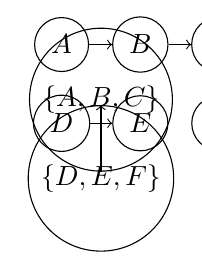
\begin{tikzpicture}
          % Equivalence classes
          \node[draw, circle] (ABC) at (1, 1) {$\{A, B, C\}$};
          \node[draw, circle] (DEF) at (1, 0) {$\{D, E, F\}$};
        
          % Edges between equivalence classes
          \draw[->] (ABC) -- (DEF);
          
          % Original Graph (Overlay)
          \begin{scope}[overlay]
            % Vertices
            \foreach \pos/\name in {{(0.5,1.7)/A}, {(1.5,1.7)/B}, {(2.5,1.7)/C}, {(0.5,0.7)/D}, {(1.5,0.7)/E}, {(2.5,0.7)/F}} {
              \node[draw, circle] (\name) at \pos {$\name$};
            }
            % Edges
            \foreach \source/\target in {A/B, B/C, D/E} {
              \draw[->, overlay] (\source) -- (\target);
            }
          \end{scope}
        \end{tikzpicture}
        \caption{Superposition d'un arbre avec son quotient}
    \end{figure}
\end{example}

Les arbres d'entités représentent l'information importante et sont donc la base de comparaison des sous arbres.
La langue naturelle contient souvent de l'information implicite ou manquante, deux sous arbres peuvent contenir un ensemble différent d'arbres d'entités, mais quand même représenter le même objet.
Par exemple, un traitement ne contient pas toujours une fréquence.
De plus la langue naturelle est ambiguë et un même ensemble d'arbres d'entités peux représenter deux objets différents.
L'ensemble seule des arbres d'entités présent dans chacun des sous arbres n'est donc pas suffisant pour déterminer leur équivalence et on doit aussi prendre en compte le contexte.
Pour ce faire nous utilisons le concept d'équivalence régulière comme introduite par~\cite{whiteGraphSemigroupHomomorphisms1983} pour les graphes.
L'idée est que deux sommets d'un graphe sont jugé équivalents si leur voisinage est équivalent.
Par exemple, deux personnes peuvent être jugées équivalent (comme catégorie d'objet représenté, ici un patient) s'ils sont toutes les deux lié à des sommets équivalents comme une maladie, un traitement, etc sans pour autant que ce soit les mêmes nœuds.

Afin de définir la relation d'équivalence nécessaire au calcul du quotient, nous définissons une mesure de similarité entre deux sous arbres.
Une mesure de similarité est une fonction symétrique $f : D \times D \to [0,1]$ où $f(x, x) = 1$ pour tout $x \in D$.
Notre similarité contextuelle, notée $sim_f(x, y)$, entre deux sous arbres enrichis $x$ et $y$, est définie comme une moyenne pondérée des similarités donnée récursivement par la fonction $f$ pour chaque sous arbre parent.
Les poids sont inversement proportionnels à la distance entre le parent et le sous arbre de départ.
Plusieurs mesures $f$ de similarité peuvent être utilisés comme Jaccard, Levenshtein, Jaro, etc.
La mesure $sim_f(x, y)$ est donné par l'équation~\ref{eq:struct:sim} où $D_{min}$ est la profondeur minimum entre les sous arbres $x$ et $y$ et $P^x_i$ (respectivement $P^y_i$) est le $i$-éme sous arbre parent de $x$ (respectivement $y$).

\begin{equation}
    sim_f(x, y) = \frac{\sum_{i=1}^{D_{min}} \frac{1}{i} \cdot f(P^x_i, P^y_i)}{\sum_{j=1}^{D_{min}} \frac{1}{j}} \label{eq:struct:sim}
\end{equation}

\begin{definition}[Equivalence de sous arbres]
    Étant donné deux arbres enrichis $T_1$ et $T_2$ et deux sous arbres respectifs $st_1 = T_1|_u$ et $st_2 = T_2|_v$.
    On dit que $st_1$ et $st_2$ sont $\tau$-similaires, noté $st_1 \sim_\tau st_2$, si $sim_f(st_1, st_2) \geq \tau$. $\sim_\tau$ est une relation réflexive et symétrique.
    La $\tau$-équivalence entre $st_1$ et $st_2$, noté $st_1 \equiv_\tau st_2$ est dérivé de la $\tau$-similarité. La relation $\equiv_\tau$ est réflexive, symétrique et transitive tel que :

    \[
        X \equiv_\tau Y \iff X \sim_\tau Z \mid \forall Z \equiv_\tau Y
    \]

    On note $[x]_\tau$ l'ensemble $\tau$-équivalent de $x$ (partition ou classe d'équivalence) donné par la clôture transitive de $\equiv_\tau$ tel que $y \in [x]_\tau \iff y \equiv_\tau x$.
    $S/\equiv_\tau$ est l'ensemble quotient (ou partitionnement) de $S$ par $\equiv_\tau$ tel que $S/\equiv_\tau = \{[x] \mid x \in S\}$, c-à-d. que $S/\equiv_\tau$ est l'ensemble de tous les ensembles $\tau$-équivalent de $S$.
    Le partitionnement d'un ensemble peut être calculé à l'aide d'un partitionnement hiérarchique en lien simple par $sim_f$ \cite{carlssonCharacterizationStabilityConvergence2010}.
\end{definition}

\todo{Explication succincte du partitionnement hiérarchique avec un exemple de dendrogramme}
